\documentclass[11pt]{article}

\usepackage[a4paper, margin=1in]{geometry}
\usepackage{setspace}
\usepackage{titlesec}
\usepackage{amsmath}
\usepackage{microtype}
\usepackage{enumitem}
\usepackage{hyperref}
\usepackage{tikz}
\usetikzlibrary{arrows.meta, positioning}

\titleformat{\section}{\large\bfseries}{\thesection}{1em}{}

\title{Monthly Return Prediction with CatBoost and Residual CNN}
\author{Aarush Ram Anandh \\ Tanush Seal}
\date{8 April 2026}

\begin{document}

\maketitle
\onehalfspacing
\setlength{\parindent}{0pt}
\setlength{\parskip}{0.4em}
\setlist[itemize]{leftmargin=1.2em}

\section{Introduction}

This project studies the prediction of gross monthly return of a company using historical factor data. Each observation is a company--month pair, with features available up to time $t$ and target $y_{i,t}$ at the same month.

The problem is challenging due to noise, non-stationarity, and missing data. Linear models fail to capture structure, while standard neural networks struggle with tabular inputs.

The approach is a two-stage model. CatBoost is first used to model cross-sectional feature relationships. The remaining error is then modeled with a temporal CNN, motivated by the hypothesis that residuals still carry short-term structure.

This yields a residual-learning pipeline: CatBoost for the base prediction and a CNN for residual correction.

\section{Methodology}

\subsection{Problem Setup}

Let $i$ denote a company and $t$ denote a month. Features are constructed using only past and current information. The goal is to predict the gross return $y_{i,t}$.

\subsection{Features and Preprocessing}

Features include financial variables and factor labels such as size, value, profitability, investment, and momentum.

All preprocessing is time-safe. Data is sorted by time, and lagged returns (1, 3, 6 months) and rolling statistics are derived from past values only. Missing values are preserved and explicitly encoded.

Time is encoded via a monotone month index and used for ordering and feature construction.

\subsection{Model}

The final prediction is:

\[
\hat{y}_{i,t} = f_{\text{CB}}(x_{i,t}) + f_{\text{CNN}}(S_{i,t})
\]

CatBoost models cross-sectional relationships, while the CNN models residual sequences of length 6.

\subsection{Training Setup}

A strict time-based split is used. The test set does not include target values.

CatBoost is trained on training data. The CNN is trained on validation residuals.

Company 194 is excluded and used as a separate holdout.

\section{Experiments and Results}

\subsection{Setup}

Evaluation is performed using time-based splits. No company split is used.

Processed data is stored in \texttt{processed\_data/}. Results are visualized in
\texttt{testing results company wise/} and \texttt{impliment.ipynb}.

\subsection{Results}

Three models are compared: CatBoost, CNN, and the combined model.

The combined model performs best. CatBoost captures overall structure, while the CNN improves short-term alignment.

However, predictions often closely follow actual values, even capturing small fluctuations.

\section{Discussion}

The results appear strong but somewhat suspicious.

Financial returns are typically noisy and difficult to predict. The observed alignment suggests possible data leakage.

Potential sources include:
- time as a categorical feature,
- residual modeling pipeline,
- shared timeline across companies.

It is also possible that strong features explain performance, but leakage seems more likely.

There may also be bias due to unfamiliarity with this type of data.

Future work involves auditing the pipeline, removing time-related features, and simplifying the model.

\section{Pipeline Overview}

\begin{center}
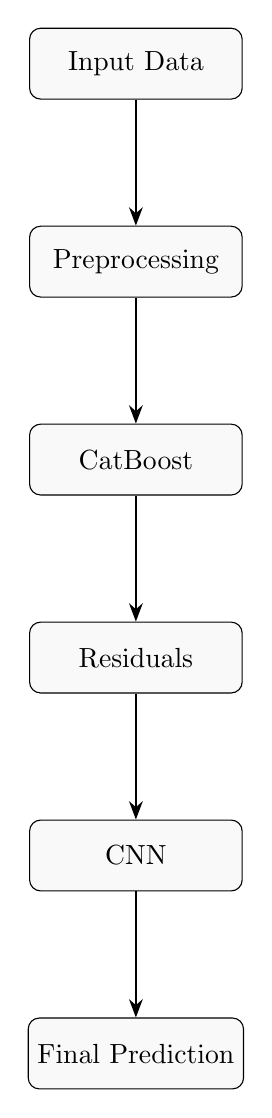
\begin{tikzpicture}[
    node distance=1.6cm,
    every node/.style={draw, rectangle, rounded corners, align=center, minimum width=2.7cm, minimum height=0.9cm, fill=gray!5},
    arrow/.style={-Stealth, thick}
]

\node (data) {Input Data};
\node (prep) [below=of data] {Preprocessing};
\node (cb) [below=of prep] {CatBoost};
\node (res) [below=of cb] {Residuals};
\node (cnn) [below=of res] {CNN};
\node (out) [below=of cnn] {Final Prediction};

\draw[arrow] (data) -- (prep);
\draw[arrow] (prep) -- (cb);
\draw[arrow] (cb) -- (res);
\draw[arrow] (res) -- (cnn);
\draw[arrow] (cnn) -- (out);

\end{tikzpicture}
\end{center}

\end{document}